\documentclass{article}

\usepackage{amsmath}
\usepackage[spanish]{babel}
\usepackage[margin=1.5in]{geometry}
\usepackage{graphicx}
\usepackage{hyperref}
\hypersetup{
    colorlinks,
    citecolor=black,
    filecolor=black,
    linkcolor=black,
    urlcolor=black,
}

\title{Apuntes prácticos de Física I A (62.01) \\ Cátedra Menikheim \\ 1° C 2004}
\author{Darío Eduardo Ramos}

\begin{document}
\maketitle
\tableofcontents{}
\newpage

\section{Requisitos para informes de trabajos prácticos}

\begin{enumerate}
\item \textbf{Carátula} con título del TP, materia y número de curso, profesor, número de grupo, integrantes, fecha de realización, fecha de entrega y de re-entregas, si hay.
\item \textbf{Resumen:} Alrededor de 8 renglones que resuman lo hecho y los resultados obtenidos. Debe ser conciso y comprensible para cualquier lector.
\item \textbf{Objetivos:} Concretos y puntuales. Generales. Deben estar narrados, no esquematizados.
\item \textbf{Descripción de los elementos utilizados:} Listado de los mismos.
\item \textbf{Introducción teórica:} Conceptos necesarios para el TP.
\item \textbf{Desarrollo/procedimiento:} Lo que se hizo, narrado con detalle. Criterios empleados, esquemas de los dispositivos empleado, fórmulas aplicadas.
\item \textbf{Resultados y discusión:} Además de presentar los resultados en sí, debe haber un análisis profundo de los mismos.
\item \textbf{Conclusiones:} Sobre el TP, sobre el tema analizado, etc.
\item \textbf{Apéndices:} Información concreta que, por su especificidad o complejidad, entorpecerían la lectura de estar en el cuerpo del informe.
\item \textbf{Bibliografía.}
\end{enumerate}

La hoja con las mediciones debe estar firmada por los docentes y entregada junto al informe.

\section{Mediciones e incertezas}

Las mediciones pueden clasificarse en:

\begin{itemize}
\item \textbf{Directas:} Se realizan con un instrumento.
\item \textbf{Indirectas:} Se emplean fórmulas algebraicas cuyos valores provienen de mediciones directas.
\end{itemize}

En términos generales, las mediciones no son exactas. Por más que se perfeccionen los métodos de medición, la discontinuidad de la materia y otros muchos factores introducen incertezas en toda medición. Por lo tanto, en el ámbito ingenieril, siempre es preferible expresar el resultado de una medición como un rango de valores que como un solo valor.

\begin{figure}[ht]
\caption{Incerteza}
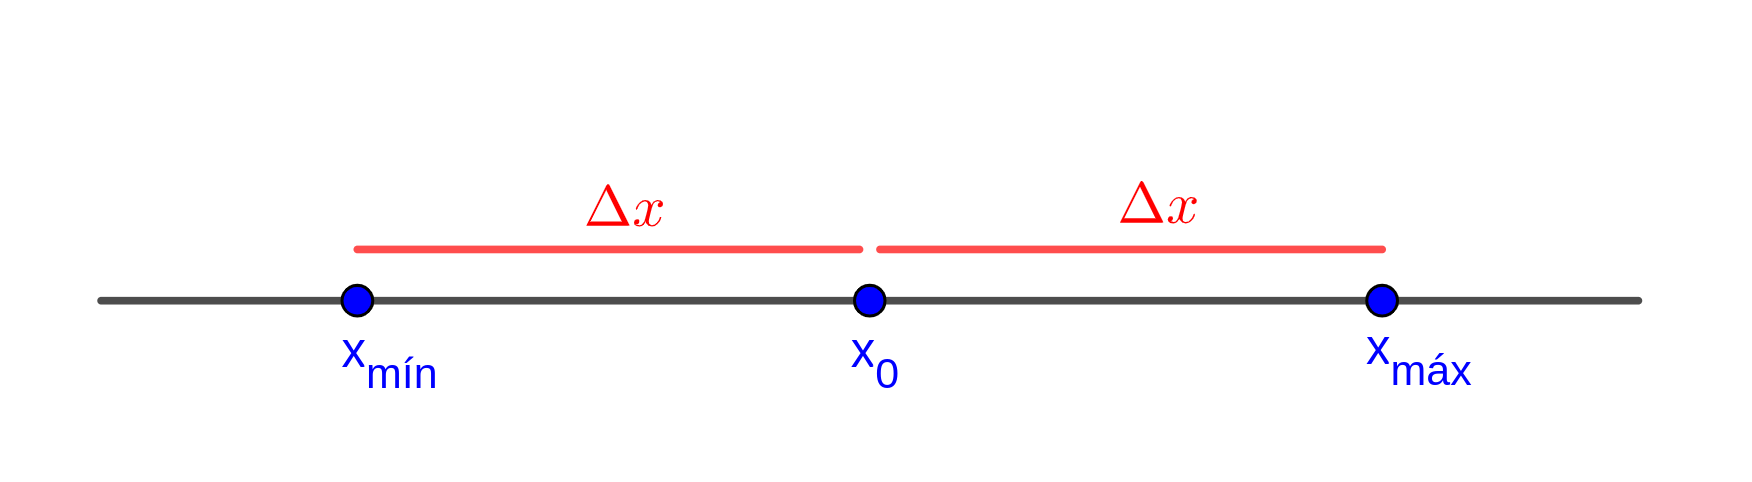
\includegraphics[scale=2]{../../common/img/62.01/practice/001-uncertainty.png} 
\centering
\label{fig:incerteza}
\end{figure}

Observando la figura \ref{fig:incerteza}, se tiene:

\begin{itemize}
\item \textbf{Valor exacto}: $x$
\item \textbf{Valor representativo}: $x_0 = \frac{x_{max} + x_{min}}{2}$
\item \textbf{Incerteza absoluta:} $\Delta x = \frac{x_{max} - x_{min}}{2}$
\item \textbf{Incerteza relativa:} $\epsilon_r = \frac{\Delta x}{x_0}$ de 0 a 1, o bien $\epsilon_{r_{\%}} = \frac{\Delta x \cdot 100}{x_0}$ si se quiere expresar como porcentaje.
\end{itemize}

Resulta entonces un valor medido expresado con incerteza:

\begin{equation}
x = x_0 \pm \Delta x
\end{equation}

Hay muchos tipos de incerteza que determinan la incerteza total. Una forma de modelarla es la siguiente:

\begin{equation}
\Delta x = \Delta L + \Delta C
\end{equation}

En este modelo, $\Delta L$ es la incerteza de lectura, asociada a errores de paralaje y limitaciones de la visión humana. Por otro lado, $\Delta C$ es la incerteza de clase de instrumento y depende del instrumento utilizado. Usualmente, se busca que $\Delta L ~ \Delta C$.

\subsection{Propagación de errores}

Al realizar operaciones aritméticas con valores inciertos, la incerteza se va propagando. Esto se verá con más detalle en Análisis Numérico (75.12), pero se hará un abordaje inicial aquí.

\subsubsection{Método tradicional}

Para la suma y la adición, se suman los errores absolutos. Para el producto y la división, se suman los errores relativos. Para la potenciación por una constante, se multiplica el error relativo por dicha constante. Es importante que si los valores tienen distinta cantidad de dígitos significativos, hay que expresar el resultado con la cantidad de dígitos significativos del operando que menos tenga. Dicho redondeo sólo se hace al final, porque redondear en cada paso intermedio aumentaría la incerteza. Además, el error se redondea primero.

\begin{subequations}
\begin{align}
\Delta (a + b) &= \Delta a + \Delta b \\
\Delta (a - b) &= \Delta a + \Delta b \\
\epsilon_r (a \cdot b) &= \epsilon_{r_a} + \epsilon_{r_b} \\
\epsilon_r \left( \frac{a}{b} \right) &= \epsilon_{r_a} + \epsilon_{r_b} \\
\epsilon_r (a^n) &= n \cdot \epsilon_{r_a}
\end{align}
\end{subequations}

\subsubsection{Método moderno}

Sea $y = f(x_1, x_2, \dots , x_n)$ una función de $n$ variables, cada una de las cuales tiene su incerteza absoluta $\Delta x_i$. Es posible demostrar entonces que:

\begin{equation}
\Delta y = \sqrt{ \left( \frac{\partial y}{\partial x_1}(x_{1_0}) \cdot \Delta x_1 \right)^2 + \left( \frac{\partial y}{\partial x_2}(x_{2_0}) \cdot \Delta x_2 \right)^2 + \ldots + \left( \frac{\partial y}{\partial x_n}(x_{n_0}) \cdot \Delta x_n \right)^2 }
\end{equation}

Nótese que las derivadas parciales están evaluadas en los valores representativos $x_{i_0}$. Aplicando la desigualdad triangular:

\begin{equation}
\Delta y \leq \left| \frac{\partial y}{\partial x_1}(x_{1_0}) \right| \Delta x_1 + \left| \frac{\partial y}{\partial x_2}(x_{2_0}) \right| \Delta x_2 + \ldots + \left| \frac{\partial y}{\partial x_n}(x_{n_0}) \right| \Delta x_n
\end{equation}

Dado que para la incerteza siempre interesan cotas superiores, el $\leq$ pasa a ser $=$ para fines prácticos. Por último, el método tradicional lleva a idénticos resultados que el moderno. Sin embargo, el segundo es más poderoso ya que permite incorporar funciones trascendentes en los cálculos.

\end{document}